\chapter{BIOMOLECULAR SIMULATION: SAMPLING AND FREE ENERGY}
\label{ch2}

All of the simulation models discussed in Chapter \ref{ch1} use an electrostatic
equation dealing with charges interacting in a vacuum. However, biological
chemistry occurs almost exclusively in an aqueous environment, necessitating the
development of models capable of simulating these systems in solution.  In this
chapter, I will describe the various methods by which solvent effects are
introduced into simulation, followed by the ensemble sampling techniques that
will be used for the principle studies in this dissertation.

\section{Simulations in the Condensed Phase}

The techniques by which solvation effects can be incorporated into various
computational models can be separated into two groups. The most obvious way is
to include the solvent atoms and molecules directly into the simulation
alongside the system of interest---referred to collectively as \emph{explicit
solvent} methods. While explicit solvent models are the most accurate approach
in principle, they drastically increase the size of the system---simultaneously
increasing the cost of the simulation and amount of sampling required to obtain
converged results.

An alternative way to include solvent effects is by modifying the electrostatic
interactions in a system to account for the natural screening that a particular
solvent provides. These approaches are called \emph{implicit solvent} methods
because solvent effects are included in an average way without including the
actual solvent atoms or molecules in the simulation. Simulations employing
implicit solvent models result in smaller systems in which comformational
sampling converges more rapidly because the solvent degrees of freedom are
already included in a mean field way. However, individual solvent molecules
often play a critical role in the structure and function of biological molecules
and behave very differently from molecules in bulk solvent---an effect implicit
solvent models are ill-equipped to handle.

The following sections describe the various implicit and explicit solvent models
commonly used in biomolecular simulations.

\subsection{Implicit Solvent}

One of the most important qualities of a solvent---especially an aqueous
solvent---is its ability to polarize in response to an electric field, thereby
reducing the magnitude of electrostatic interactions across a given distance.
While the na\"ive approach of simply applying the solvent dielectric everywhere
is attractive in its simplicity, solvent-excluded regions should obviously not
be subject to the screening effects of the solvent. For large biomolecules, the
solvent-excluded regions can be quite large, so it becomes important to deal
with these regions effectively.

\subsubsection{Distance-dependent Dielectric}

Among the earliest approaches to account for the different dielectric
environments of the interior of a bimolecule and bulk solvent introduced a
dielectric constant that changed as a function of the distance between two
charged particles. As the separation between two particles increased, so too did
the likelihood that they were separated by solvent, and were therefore subject
to dielectric screening effects.

This approach is attractive in its simplicity---it adds little to the
computational cost of the model while retaining the simple,
pairwise-decomposable nature of the electrostatic potential term. A common
equation modeling the dielectric constant is given below in Eq.
\ref{eq2:DistanceDielectric}. \cite{Leach_Book_MolModel_2001}

\begin{equation}
   \varepsilon _ {eff} (r) = \frac {\varepsilon_{bulk} - 1} 2 \left [ (rS) ^2 +
   2rS + 2 \right ] \exp(-rS)
   \label{eq2:DistanceDielectric}
\end{equation}
where $r$ is the distance between the two particles, $\varepsilon_{bulk}$ is the
dielectric constant of the bulk, $\varepsilon_{eff}$ is the effective
dielectric constant at a given particle separation, and $S$ is a free parameter.
Fig. \ref{fig2:DistanceDielectric} plots the resulting curve for
$\varepsilon_{eff}$ from Eq. \ref{eq2:DistanceDielectric} for different values
of the free parameter.

\begin{figure}
   \includegraphics[width=6.5in]{DistanceDielectric.ps}
   \caption{Distance-dependent dielectric for different values of the free
            parameter $S$ in Eq. \ref{eq2:DistanceDielectric}.}
   \label{fig2:DistanceDielectric}
\end{figure}

This effective dielectric constant is then incorporated as $\epsilon$ in Eq.
\ref{eq1:AmberFF2}, and influences the calculated forces due to its dependence
on $r_{i,j}$. One of the biggest weaknesses of distance-dependent
dielectrics is that it treats every atom in the biomolecule as though they are
in the same environment, whereas the shapes of biomolecules---and their
solvent-excluded volumes---are often highly irregular. That is, two atoms buried
inside the solvent-excluded volume separated by $d$ {\AA} are treated exactly
the same way as two different atoms $d$ {\AA} apart whose interstitial region is
solvent-accessible. Furthermore, because the shapes of biomolecules can vary
greatly from system to system, the `optimal' value for $S$ in Eq.
\ref{eq2:DistanceDielectric} is highly system-dependent. Finally, while the true
dielectric regions are either the value of the bulk solvent or the molecule
interior, a distance-dependent dielectric has a large region corresponding to
unphysical, intermediate values of the dielectric.

For these reasons, the distance-dependent dielectric model is rarely used in
modern simulations, having given way to the more accurate methods like the
Poisson-Boltzmann and Generalized Born equations.

\subsubsection{Poisson-Boltzmann}

At the heart of most modern implicit solvent models lies the Poisson equation
\begin{equation*}
   \bigtriangledown \epsilon(\vec{r}) \cdot \bigtriangledown \phi ( \vec{r} ) =
            -4 \pi \rho(\vec{r})
\end{equation*}
where $\phi$ is the electrostatic potential distribution function, $\rho$ is
the charge distribution function, and $\epsilon$ is the dielectric constant at a
given point in space. The dielectric constant is often divided into two
regions---a region of low dielectric in the solvent-excluded volume and that of
the bulk solvent `outside' the system of interest.
\cite{Cramer_Book_EssentialsCompChem_2004}

The Poisson equation is only valid, however, at zero ionic strength. When mobile
ions are present---as is the case \emph{in vivo} with all biomolecules---the
Poisson equation must be augmented with an appropriate distribution of
counterions. The probability of finding an ion in a particular region of space
is related to its Boltzmann factor $\exp (-\beta q \phi(\vec{r}))$, where $q
\phi(\vec{r})$ is the energy of a point charge in a given electrostatic
potential. Because ions come in pairs with both positive and negative charges,
the Boltzmann probability of finding both types of ions must be included. The
equation for calculating the electrostatic potential in a biomolecular system
with a given solution ionic strength, termed the \emph{Poisson-Boltzmann} (PB)
equation, is shown in Eq. \ref{eq2:PoissonBoltzmann}.
\cite{Cramer_Book_EssentialsCompChem_2004}

\begin{align}
   \bigtriangledown \epsilon(\vec{r}) \cdot \bigtriangledown \phi(\vec{r}) -
      \epsilon(\vec{r}) \lambda(\vec{r}) \kappa^2 \frac{k_B T} {2 q} \exp \left
      ( -\beta q \phi(\vec{r}) \right ) + \epsilon(\vec{r}) \lambda(\vec{r})
      \kappa^2 \frac{k_B T} {2 q}  \exp \left ( \beta q \phi(\vec{r})
      \right ) & = -4 \pi \rho (\vec{r}) \nonumber \\ \bigtriangledown
      \epsilon(\vec{r}) \cdot \bigtriangledown \phi(\vec{r}) - \epsilon(\vec{r})
      \lambda(\vec{r}) \kappa^2 \frac{k_B T} q \sinh \left ( \frac {q
      \phi(\vec{r})} {k_B T} \right ) & = -4 \pi \rho (\vec{r})
   \label{eq2:PoissonBoltzmann}
\end{align}

In Eq. \ref{eq2:PoissonBoltzmann}, $q$ is the charge of the ions (both positive
and negative ions are present), $\lambda(r)$ is a simple switching function that
is 0 in solvent-excluded regions and 1 in solvent-accessible regions, and
$\kappa^2$ is related to the ionic strength as
\begin{equation*}
   \kappa ^ 2 = \frac {8 \pi q ^ 2 I} {\epsilon k_B T}
\end{equation*}

Eq. \ref{eq2:PoissonBoltzmann} is a non-linear, second-order differential
equation in the electrostatic potential that must be solved iteratively until
the desired level of self-consistency in the electrostatic potential is
achieved. The $\sinh$ term in Eq. \ref{eq2:PoissonBoltzmann} may be expanded
using its Taylor series expansion. If the ionic strength is low and the solute
is not highly charged (so $\phi(\vec{r})$ is relatively small), the Taylor
series expansion for $\sinh$ can be truncated after the first term to yield the
much simpler Eq. \ref{eq2:LinearPB} with little loss of accuracy. Eq.
\ref{eq2:LinearPB} is called the \emph{linearized} Poisson-Boltzmann equation
because the Taylor series expansion for $\sinh$ is truncated after its linear
term.

\begin{equation}
   \bigtriangledown \epsilon (\vec{r}) \bigtriangledown \phi(\vec{r}) -
         \epsilon(\vec{r}) \lambda(\vec{r}) \kappa ^ 2 \phi(\vec{r}) = -4 \pi
         \rho(\vec{r})
   \label{eq2:LinearPB}
\end{equation}

The Poisson Equation can be solved exactly for only the simplest systems, like
solvating a point-charge or a conducting sphere with a uniform charge
distribution on its surface. Eq. \ref{eq2:PoissonBoltzmann} or
\ref{eq2:LinearPB} must be solved numerically for complex biomolecules with
irregular shapes. A common approach is to set up a three-dimensional grid
surrounding the solute and calculate the charge distribution on the grid from
the partial charges of each solute atom.  The dielectric boundary can be
calculated from the solvent accessible surface
\cite{Sitkoff_JPhysChem_1994_v98_p1978}, so each grid point has an associated
charge and dielectric value. The differential equations can then be solved via
finite differences within the defined grid. \cite{Klapper_Proteins_1986_v1_p47}

After the electrostatic potential is calculated via Eq.
\ref{eq2:PoissonBoltzmann}, the free energy is calculated by integrating the
product of the charge distribution and the calculated electrostatic potential
according to
\begin{equation*}
   G = \frac 1 2 \int \rho(\vec{r}) \phi(\vec{r}) d\vec{r}
\end{equation*}
where the $1/2$ factor corrects for double-counting the interactions.  The free
energy of solvation due to solvent polarization is calculated from the
difference in the electrostatic potentials in vacuum and solvent ($\phi_{solv} -
\phi_{vac}$)---a quantity referred to as the \emph{reaction field}.
\cite{Leach_Book_MolModel_2001} The charge-dependent portion of the solvation
free energy then becomes
\begin{equation}
   \Delta G _ {pol} = \frac 1 2 \int \rho(\vec{r}) \left ( \phi_{solv}(\vec{r})
      - \phi_{vac}(\vec{r}) \right ) d\vec{r}
   \label{eq2:ReactionField}
\end{equation}

Models employing implicit solvent via the PB equation have proven
effective in many cases. \cite{Klapper_Proteins_1986_v1_p47,
Gilson_JComputChem_1988_v9_p327, Baker_ProcNatlAcadSci_2001_v98_p10037,
Nielsen_Proteins_2001_v43_p403} However, due to requirements of a fairly dense
grid and the iterative, self-consistent nature of solving the PB equation, the
computational cost of this model is too high for many applications. Furthermore,
the dielectric function is discontinuous at the boundaries of the
solvent-excluded and solvent-accessible regions, making stable gradients (and
therefore forces) difficult to calculate.
\cite{Wang_ChemPhysLett_2009_v468_p112} Therefore, I will now consider a common
approximation to the PB equation called the \emph{Generalized Born} model that
seeks to provide an efficient, analytical alternative to solving the PB
equation.

\subsubsection{Generalized Born}

While the electrostatic potential generated by most charged species cannot be
solved analytically using the Poisson equation, I will consider two simple,
ideal systems that can. The first is a perfect conducting sphere of radius $r$
with a uniform charge distribution. Given a total charge $q$ and using the
Poisson equation to calculate the electrostatic potential induced by the charged
sphere, the polar contribution to the free energy of solvation can be calculated
from Eq. \ref{eq2:ReactionField}, giving the familiar \emph{Born} equation,
shown below. \cite{Cramer_Book_EssentialsCompChem_2004}
\begin{equation}
   \Delta G _ {pol} = - \frac 1 2 \left( \frac 1 {\epsilon_{vac}} - \frac 1
         {\epsilon_{bulk}} \right) \frac {q ^ 2} r
   \label{eq2:Born}
\end{equation}
In Eq. \ref{eq2:Born}, $\epsilon_{vac}$ is the dielectric constant of a vacuum,
which is unity.  It is shown explicitly here to demonstrate that the dielectric
constant of the solvent-excluded volume in the Poisson equation does not appear
in the Born equation.

If instead of being a perfect conducting sphere with a uniform charge
distribution, the sphere had a perfect dipolar charge distribution, the free
energy of solvation using the Poisson equation would result in the
\emph{Kirkwood-Onsager} equation, shown below.
\cite{Cramer_Book_EssentialsCompChem_2004}
\begin{equation}
   \Delta G _ {pol} = - \frac 1 2 \left ( \frac {2 ( \epsilon - 1 )} {2 \epsilon
         + 1} \right ) \frac {\mu ^ 2} {r ^ 3}
   \label{eq2:KirkwoodOnsager}
\end{equation}
where the $\epsilon$ is the dielectric constant of the bulk solvent and the
dielectric constant of vacuum has simply been replaced by 1.

The \emph{Generalized Born} (GB) formalism for calculating the polar
contribution to the solvation free energy is, as its name would suggest, an
extension of the \emph{Born} solution shown in Eq. \ref{eq2:Born} to complex
molecules with an arbitrary size and shape.
\cite{Still_JAmChemSoc_1990_v112_p6127, Qiu_JPhysChemA_1997_v101_p3005,
Onufriev_JPhysChemB_2000_v104_p3712, Bashford_AnnuRevPhysChem_2000_v51_p129,
Onufriev_JComputChem_2002_v23_p1297}
\citeauthor{Still_JAmChemSoc_1990_v112_p6127} was the first to propose the
method, adjusting the Born equation (Eq. \ref{eq2:Born}) as shown below.
\cite{Still_JAmChemSoc_1990_v112_p6127}
\begin{equation}
   \Delta G _ {pol} = -\frac 1 2 \left( 1 - \frac 1 {\epsilon} \right)
      \sum_{i=1}^N \sum_{j=1}^N \frac {q_i q_j} {f_{GB}}
   \label{eq2:GB}
\end{equation}
where $q_i$ is the charge of atom $i$, $\epsilon$ is the dielectric constant of
the solvent, and $f_{GB}$ is an arbitrary, analytic function of atom positions
designed to calibrate Eq. \ref{eq2:GB} to experiment. The most common form of
$f_{GB}$ devised by \citeauthor{Still_JAmChemSoc_1990_v112_p6127}, and still
used predominantly today, is shown in Eq. \ref{eq2:fGB}.

\begin{equation}
   f_{GB} = \sqrt{r_{i,j}^2 + \alpha_i \alpha_j \exp \left( - \frac {r_{i,j}^2}
            {4 \alpha_i \alpha_j} \right)}
   \label{eq2:fGB}
\end{equation}
where $r_{i,j}$ is the distance between atoms $i$ and $j$ and $\alpha_i$ is
called the effective Born radius of atom $i$ for reasons that will soon be
apparent.

Eq. \ref{eq2:fGB} does not represent a theoretically `correct' choice for
$f_{GB}$, nor has it been shown to be the best choice---in fact it probably is
not. \cite{Onufriev_JChemPhys_2011_v134_p164104} However, it is a good choice
for several reasons. First, Eq. \ref{eq2:fGB} is a simple formula with
analytical gradients---assuming $\alpha_i$ is an analytic function of the
nuclear positions---and can be computed rapidly. More importantly, however, Eq.
\ref{eq2:fGB} has the appropriate limiting behavior.
\cite{Still_JAmChemSoc_1990_v112_p6127} For a single particle---or two identical
point charges separated by a distance of 0---$f_{GB}$ reduces to $\alpha$ and
Eq. \ref{eq2:GB} reduces to the Born equation (Eq. \ref{eq2:Born}) in which the
radius of the `sphere' is $\alpha_i$. It is for this reason that the $\alpha_i$
values can be thought of as an `effective' radius. Furthermore, for two point
charges separated by a small distance (\ie smaller than the effective radii of
the two particles) the result agrees with the Kirkwood-Onsager solution (Eq.
\ref{eq2:KirkwoodOnsager}) to within 10\% of the true value.
\cite{Still_JAmChemSoc_1990_v112_p6127}

The next major challenge in solving Eq. \ref{eq2:GB} is calculating the
effective Born radii, $\alpha_i$, for each atom. The effective radius of an atom
reflects the spherically average distance of that atom from the solvent excluded
surface. Calculating the effective radii is particularly challenging because it
must be done rapidly, accurately, and so gradients may be easily computed.
Because GB was developed as an efficient alternative to solving the PB equation,
computationally intensive approaches to calculating the effective radii offer
little advantage over using the more precise PB equation. Furthermore,
\citeauthor{Onufriev_JComputChem_2002_v23_p1297} has demonstrated the importance
of computing effective Born radii accurately,
\cite{Onufriev_JComputChem_2002_v23_p1297} showing that so-called `perfect
radii' reproduce PB results very closely. Finally, gradients are necessary to
perform either geometry optimization or molecular dynamics, and an expression
that lends itself to rapid computation of an accurate gradient is an attractive
feature.

The most common approach to computing the effective radius is called the
\emph{coulomb field approximation}, shown below in Eq. \ref{eq2:CFA}.
\cite{Cramer_Book_EssentialsCompChem_2004}

\begin{equation}
   I _ i = \int _ {\Omega_i} \frac {d^3r} {4 \pi r ^ 4}
   \label{eq2:CFA}
\end{equation}

$I_i$ in Eq. \ref{eq2:CFA} is the coulomb field integral for atom $i$ and
$\Omega_i$ signifies the integral is over all space centered on atom $i$. The
effective radius is then computed from this integral using Eq. \ref{eq2:reff}.

\begin{equation}
   \alpha _ {i} = \left( \rho _ i ^ {-1} - I _ i \right) ^ {-1}
   \label{eq2:reff}
\end{equation}
where $\rho_i$ is the intrinsic van der Waals radius of atom $i$ and $I_i$ is
the integral from Eq. \ref{eq2:CFA}.

As computational power increased and simulations reached longer time scales and
larger systems, however, deficiencies in these equations began to surface,
leading to efforts to improve the calculation of the effective Born radii.
\cite{Onufriev_JComputChem_2002_v23_p1297, Onufriev_Proteins_2004_v55_p383,
Mongan_JChemTheoryComput_2007_v3_p156, Nguyen_JChemTheoryComput_2013_ASAP} The
two approaches that have been implemented in the Amber suite of programs are
briefly described below.

\citeauthor{Onufriev_Proteins_2004_v55_p383} noticed that Eqs. \ref{eq2:CFA} and
\ref{eq2:reff} tended to underestimate the effective radii of buried atoms
because it assumed that interstitial regions of space between atoms were
solvent-filled, despite the fact that they were too small to contain a full
water molecule. \cite{Onufriev_Proteins_2004_v55_p383} As a result, they
modified Eq. \ref{eq2:reff} into the following form:
\begin{equation}
   \alpha _ i = \left[ \rho _ i ^ {-1} - \rho _ i ^ {-1} \tanh \left( a
   \Psi - \beta \Psi^2 + \gamma \Psi^3 \right) \right] ^ {-1}
   \label{eq2:reffOBC}
\end{equation}
where $\Psi = I \rho_i$ ($I_i$ is taken from Eq. \ref{eq2:CFA}), and $a$,
$\beta$, and $\gamma$ are fitting parameters. The $\tanh$ function was chosen
because it is infinitely differentiable (analytically) and increases the
effective radii of more deeply-buried atoms while leaving the effective radii of
atoms closer to the surface unchanged. In this way, Eq. \ref{eq2:reffOBC}
maintains the success Eq. \ref{eq2:reff} displayed for small compounds while
improving the behavior of deeply-buried residues.
\cite{Onufriev_Proteins_2004_v55_p383} This GB variant is referred to as
GB\super{OBC} (where OBC comes from the authors Onufriev, Bashford, and Case).

\citeauthor{Mongan_JChemTheoryComput_2007_v3_p156} took a different approach.
While Eq. \ref{eq2:reffOBC} provided uniform scaling for all atoms with a given
degree of burial (as measured by the value of $I_i$ in Eq. \ref{eq2:CFA}),
\citeauthor{Mongan_JChemTheoryComput_2007_v3_p156} adopted an approach based on
geometry. By treating each atom and each solvent molecule as a sphere---a good
approximation for a water molecule---the interstitial space between two solute
atoms that is inaccessible to solvent can be quantified. Because this
interstitial region resembles a neck---as seen in Fig.
\ref{fig2:Interstitial}---this model is referred to as GB\super{neck}.
\cite{Mongan_JChemTheoryComput_2007_v3_p156}

\begin{figure}
   \includegraphics[height=6.5in, angle=90, trim=1cm 0.5cm 1cm 0.5cm, clip=true]
                   {Interstitial.ps}
   \caption[Region of space between two atoms $i$ and $j$ of radius $R_i$ and
            $R_j$ that is inaccessible to a spherical solvent molecule of radius
            $R_{solv}$.]
           {Region of space between two atoms $i$ and $j$ of radius $R_i$ and
            $R_j$ that is inaccessible to a spherical solvent molecule of radius
            $R_{solv}$. This inaccessible region is called the \emph{neck} and
            is shaded gray.}
   \label{fig2:Interstitial}
\end{figure}

The most recent approach by \citeauthor{Nguyen_JChemTheoryComput_2013_ASAP}
involves a re-parametrization of the intrinsic atomic radii ($\rho_i$ in Eq.
\ref{eq2:reff}) for atoms commonly involved in salt bridges and a combination of
the ideas presented in the GB\super{OBC} and GB\super{neck} models described
above. \cite{Nguyen_JChemTheoryComput_2013_ASAP}

\subsubsection{Non-polar Solvation}

The process of solvation can be broken down into two fictitious steps---a
cavitation step in which the solvent is excluded from a region of space equal to
the solute's solvent excluded volume, and a charging step where the
solvent-polarized charge distribution of the solute is inserted into that
cavity. Because the free energy is a state function, this gedanken decomposition
will yield an identical free energy to the true experimental free
energy---assuming of course that each step can be calculated exactly.  The free
energies of these two steps are referred to as the non-polar and polar solvation
free energy, respectively.

The Poisson-Boltzmann and Generalized Born equations shown in Eqs.
\ref{eq2:PoissonBoltzmann} and \ref{eq2:GB} are used to compute the polar
solvation free energy (\ie the portion of the free energy derived from the
reaction field). There are several methods for calculating the non-polar
solvation free energy.

Methods for calculating the non-polar contribution to solvation are often
parametrized by assuming that the solvation free energy for extended and
branched alkanes is non-polar in nature. The most common way to calculate
non-polar solvation is to fit a surface tension value to the experimental
solvation free energies of the alkanes.
\cite{Cramer_Book_EssentialsCompChem_2004} This approach can be rationalized
using the idea that the presence of a non-polar solute immersed in solvent
disrupts the solvent-solvent interactions, thereby restricting solvent structure
in the solvation shell surrounding the solute. This effect imposes an entropic
penalty to solvation (that is offset by the polar solvation term for soluble
compounds).  If this was the only source of the `non-polar' solvation free
energy, then its magnitude would vary with the size of the molecule, which is
directly related to its surface area.

Combining this surface-area non-polar solvation term with either the
Poisson-Boltzmann or Generalized Born equations for the polar solvation term
results in the so-called \emph{PBSA} and \emph{GBSA} methods, respectively. One
of the most common methods for calculating the surface area in GBSA molecular
dynamics simulations is called the \emph{linear combination of pairwise
overlaps} (LCPO) method---so-called because it is parametrized by fitting five
parameters to the spherical overlaps of individual atoms.
\cite{Weiser_JComputChem_1999_v20_p217} The chief advantage of LCPO is that it
provides an efficient way to calculate surface areas using an analytical formula
whose derivatives can be easily calculated for use in molecular dynamics.

\subsection{Explicit Solvent}

While the implicit solvent methods described above are useful ways of
incorporating solvation effects in molecular simulations, all solvent effects
are accounted for in an average way. Therefore, individual water molecules that
play structurally important roles in biomolecules are not treated well by either
PB or GB methodologies. In such cases, it is advantageous to include the solvent
molecules explicitly in the simulation. Explicit solvent significantly increases
the cost of the simulation by adding a large number of atoms to the system, but
should improve the accuracy by creating a model closer to reality.

A large drawback when adding explicit solvent, however, is the fact that modern
simulations at an atomic resolution (\ie where all atoms are treated explicitly)
are limited to, at most, $10^8$ atoms, \cite{100M_Stupid} although simulations
between $10^5$ to $10^6$ atoms are more reasonable. Macroscopic systems, on the
other hand, contain on the order of $10^{23}$ atoms---an intractable number for
modern hardware, so our simulations must be scaled down to a microscopic size.

As a demonstration, the hairpin ribozyme is a biomolecule that contains roughly
\mbox{2 100} atoms. Adding only \mbox{22 000} water molecules---enough to create
a 20 {\AA} spherical solvent buffer around the ribozyme---increases the
simulation size to roughly \mbox{90 000} atoms. It is quite clear, therefore,
that even on the largest supercomputers, we can only model a microscopic droplet
in explicit solvent. At such small sizes, the ratio of surface area to volume
for these minuscule droplets is astronomically large, and water molecules at the
solvent-air interface behave quite differently from those molecules in bulk
solvent.

While early approaches of applying a `cap' potential---an artificial biasing
potential penalizing solvent that diffuses too far away from the solute---helped
overcome some surface effects like evaporation, it made direct comparison to
experiment dubious. A major breakthrough in explicit solvent calculations came
with the introduction of periodic boundary conditions. \cite{Allen_Tildesley}

\subsubsection{Periodic Boundary Conditions}

To emulate bulk solution behavior using a system composed of a tractable number
of atoms, we impose periodic boundary conditions (PBC) on the system,
replicating it infinitely in every dimension. In such a system, each atom
interacts with all other atoms in all other simulation cells---including its own
periodic images. \cite{Allen_Tildesley} A two-dimensional illustration of PBC is
shown in Fig. \ref{fig2:PBC} for a rectangular unit cell illustrating these
ideas.

A practice commonly adopted in PBC simulations in which each atom interacts
directly with only a single image of every other atom---specifically the nearest
image---is called the \emph{minimum image convention}. The minimum image
convention is employed to simplify the problem, but also imposes a limit to the
range of calculated interactions. Specifically, the non-bonded interactions do
not extend beyond half the length of the shortest side of the unit cell.
Employing the minimum image convention, the energy calculated for a system with
PBC is the energy of a single unit cell in the field generated by every periodic
cell. The challenge is how to calculate the non-bonded interactions for every
atom in the system. The common approaches employed in biomolecular simulation
are explored in the next three sections.

\begin{figure}
   \includegraphics[height=6.5in, angle=90, trim=0.7cm 3cm 0.7cm 3cm, clip=true]
                   {PBC.ps}
   \caption[Periodic simulation in two dimensions with a rectangular unit cell.
            The maximum permissible cutoff (r\sub{cut}) for the minimum image
            convention is shown]
           {Periodic simulation in two dimensions with a rectangular unit cell.
            The maximum permissible cutoff (r\sub{cut}) for the minimum image
            convention is shown with a blue dotted circle centered on particle 1
            in the first box.}
   \label{fig2:PBC}
\end{figure}

\subsubsection{Cutoff Methods}

The simplest approach to calculating non-bonded interactions is to employ a
simple cutoff that is smaller than half the length of the shortest side of the
unit cell---\ie all non-bonded interactions between atoms closer than the cutoff
are included and all those between atoms greater than the cutoff are neglected.
Because the common forms of the non-bonded potential decay as the distance
between atoms increases (see Eqs. \ref{eq1:ElectrostaticInteractions} and
\ref{eq1:LennardJones}), interactions between distant atoms are significantly
smaller than interactions between nearby atoms. The non-bonded interactions are
modeled as the simple piecewise function shown in Eq. \ref{eq2:cutoff}.

\begin{equation}
   U^{\prime}(\vec{x}_{i,j}) = \left \{
   \begin{array}{lr}
      U(\vec{x}_{i,j}) & : \left | \vec{x}_{i,j} \right | < x_{cut} \\
      0 & : \left | \vec{x}_{i,j} \right | > x_{cut}
   \end{array}
   \right.
   \label{eq2:cutoff}
\end{equation}

While conceptually simple and computationally efficient, simple cutoffs suffer
from a severe limitation. The potential, and therefore the force, encounters a
discontinuity at the cutoff distance, shown in Fig.
\ref{fig2:Cutoff}A. This discontinuity results in simulations that do not
conserve energy and leads to numerous, non-physical artifacts.
\cite{Schreiber_JMolBiol_1992_v228_p909, Schreiber_Biochemistry_1992_v31_p5856,
Saito_JChemPhys_1994_v101_p4055, Auffinger_ChemPhysLett_1995_v234_p413,
Cheatham_JAmChemSoc_1995_v117_p4193, Feller_JPhysChem_1996_v100_p17011,
Patra_BiophysJ_2003_v84_p3636} This effect is particularly pronounced for
electrostatic interactions---a very long-range potential of the form $1/r$. As
mentioned before, this function decays so slowly that $\sum_{i=1}^{\infty} 1/r =
\infty$.  Two monovalent ions must be separated by $\sim$332 {\AA} before their
interaction energy drops to 1 kcal/mol. Such a cutoff would require a unit cell
size at least 664 {\AA} on each edge containing $\sim$10\super{7} water
molecules.

Given the need to improve the behavior of the non-bonded potentials near the
cutoff distance, two popular modifications to the simple cutoff approach were
introduced---a smooth switching function and a shifting function. The switching
function approach applies a smooth function at a given distance that satisfies
the following criteria: a) the potential and its gradient is continuous
everywhere, b) the short-ranged form of the potential is unchanged, and c) the
potential approaches 0 at the cutoff. Eq. \ref{eq2:cutoff} is an example of a
very simple switching function in which the original potential is multiplied by
1 when the interparticle distance is less than the cutoff and 0 otherwise. Of
course, this switching function does not obey either the a) or c) conditions
listed above. An example of a smooth switching function is shown in Fig.
\ref{fig2:Cutoff}B. \cite{Steinbach_JComputChem_1994_v15_p667}

The second family of methods commonly employed are so-called shifting functions
since the potential is modified by `shifting' the potential up such that the
value of the potential becomes zero at the cutoff distance.
\cite{Steinbach_JComputChem_1994_v15_p667, Allen_Tildesley} Simply shifting the
potential, though, is not enough for MD simulations, since the force will remain
unchanged and still faces a discontinuity at the cutoff. Therefore, the shifting
function often contains a force-shifting component, as shown in Eq.
\ref{eq2:ShiftingFunction}. \cite{Allen_Tildesley} The effect of the shifting
function is shown in Fig. \ref{fig2:Cutoff}C.

\begin{equation}
   U_s(\vec{r}_{i,j}) = \left\{
   \begin{array}{lr}
      U(\vec{r}_{i,j} - U(\vec{r}_{cut}) - \left( \frac {dU(\vec{r}_{i,j})}
        {d\vec{r}_{i,j}} \right) _ {\vec{r}_{i,j} = \vec{r}_{cut}}
        (\vec{r}_{i,j} - \vec{r}_{cut}) & \vec{r}_{i,j} < \vec{r}_{cut} \\
      0 & \vec{r}_{i,j} \geq \vec{r}_{cut}
   \end{array}
   \right.
   \label{eq2:ShiftingFunction}
\end{equation}

\begin{figure}
   \includegraphics[height=6.5in, angle=90]{Cutoff.ps}
   \caption[Effects of various 16 {\AA} cutoff schemes on the electrostatic
            interaction of two monovalent ions with opposite charges.]
           {Effects of various 16 {\AA} cutoff schemes on the electrostatic
            interaction of two monovalent ions with opposite charges. A) shows
            the effect of imposing a hard cutoff. B) shows a typical switching
            function starting at 8 {\AA}. C) shows a typical shifting function
            for the electrostatic potential. The energies as a function of
            distance are shown in the top 3 plots and the forces as a function
            of distance are the bottom 3 plots.}
   \label{fig2:Cutoff}
\end{figure}

\subsubsection{Ewald Summation}

Ideally, simulations in the condensed phases would be performed \emph{without}
truncating electrostatic interactions at all. The full electrostatic interaction
for a net neutral unit cell takes the functional form $\sum_{i=1}^N (-1)^i / i$,
since there are an equal number of charges of both signs. This sum is
\emph{conditionally convergent}, meaning that, while it converges to a finite
value, that value depends on the order in which the terms are summed.
\cite{Allen_Tildesley} A natural choice for ordering the summation of the
infinite number of electrostatic interactions with particle $i$ is by summing
all of the electrostatic interactions with each particle $j$ in every unit cell
extending radially from the unit cell containing $i$. This approach is shown
diagrammatically in Fig. \ref{fig2:PeriodicCells}.
\cite{Allen_Tildesley}

\begin{figure}
   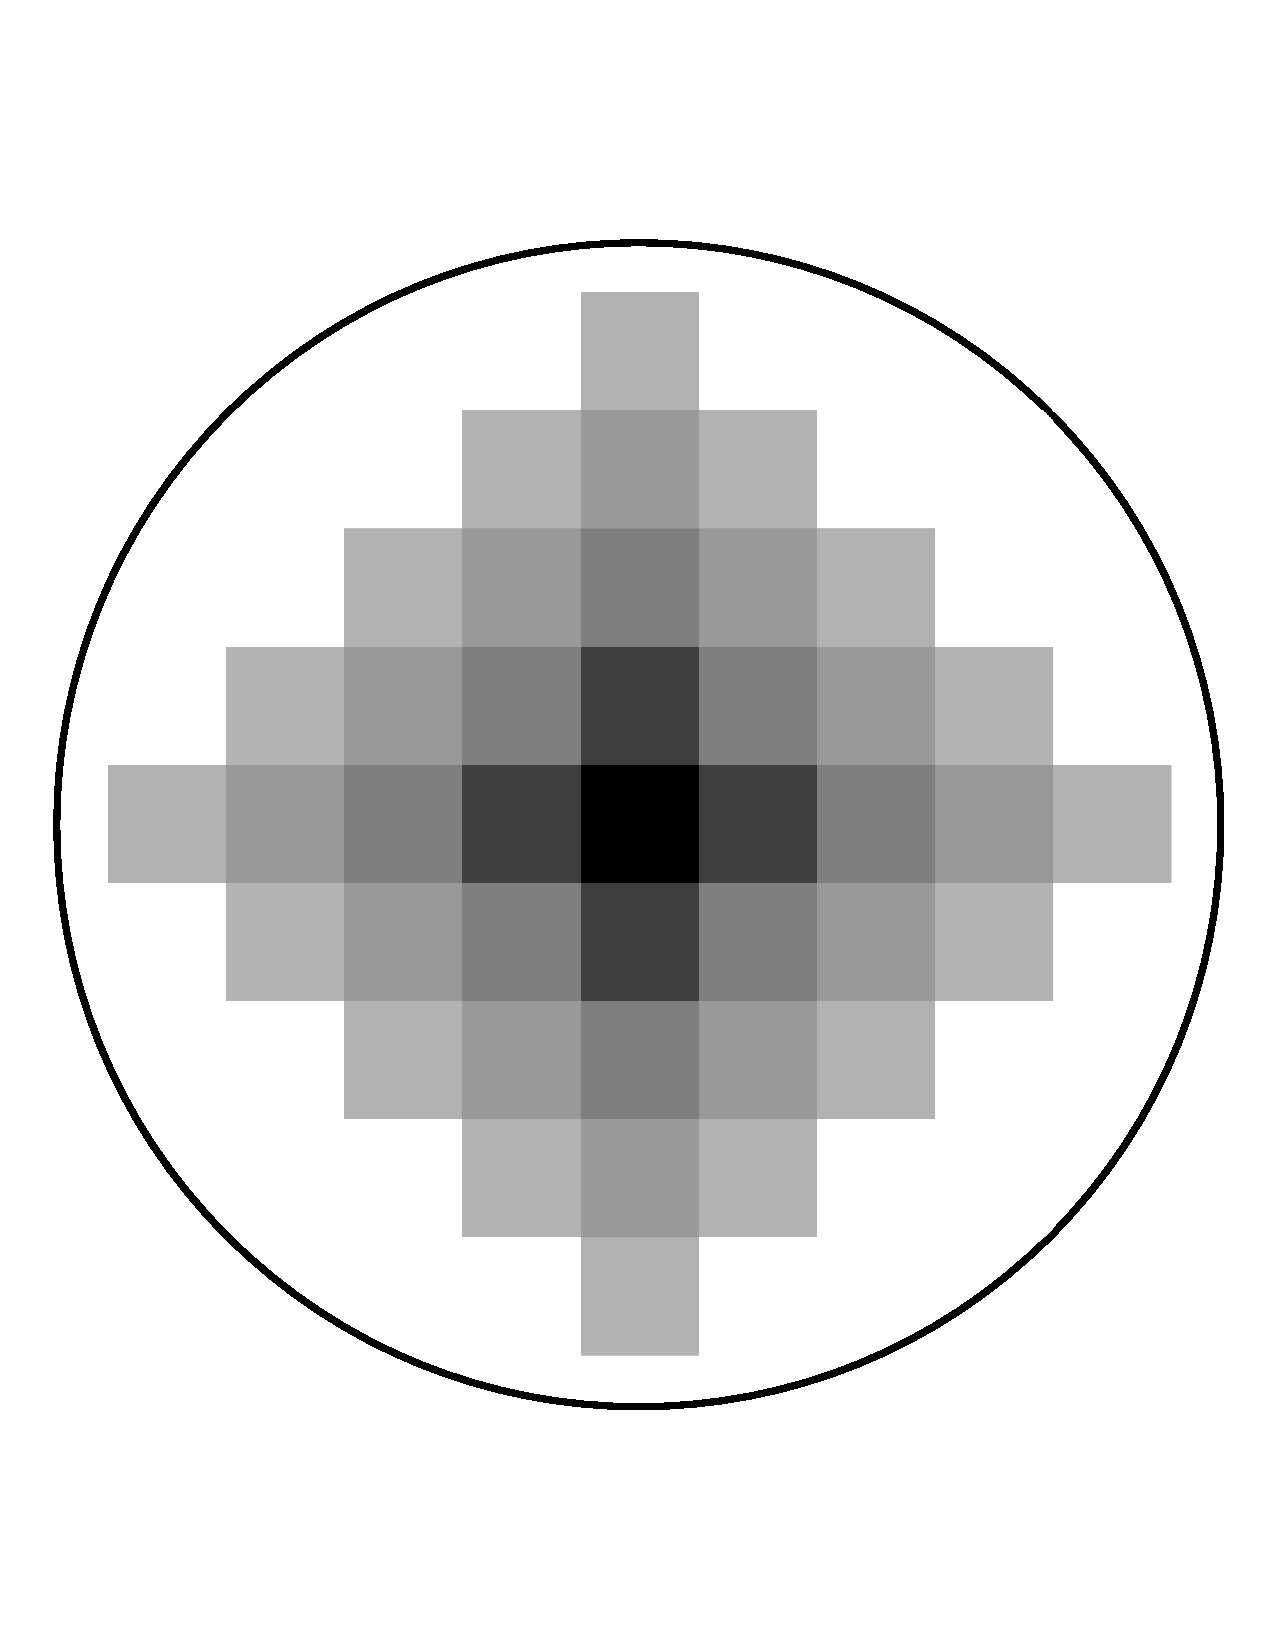
\includegraphics[height=4in, angle=90, trim=0.1cm 2cm 0.1cm 2cm, clip=true]
                    {PeriodicCells.ps}
   \caption[Periodic cells added in a spherical shape radially from the central
            unit cell. The progression from darker to lighter cells shows]
           {Periodic cells added in a spherical shape radially from the central
            unit cell. The progression from darker to lighter cells shows the
            order in which interactions are accumulated in the sum of the
            electrostatic interactions (with the darker cells being added before
            the lighter ones). The example, adapted from
            \citeauthor{Allen_Tildesley}, is shown in two dimensions, but can
            be trivially extended to three dimensions. \cite{Allen_Tildesley}}
   \label{fig2:PeriodicCells}
\end{figure}

In 1921, \citeauthor{Ewald_AnnPhys_1921_v64_p253} devised a method whereby the
electrostatic interactions between an ion and all of its periodic images in a
crystal lattice could be computed according to the technique presented in Fig.
\ref{fig2:PeriodicCells}. \cite{Ewald_AnnPhys_1921_v64_p253} The same approach
can be used for simulations in the condensed phase when PBC are used.  The
technique, called the Ewald sum, utilizes a trick to cause the electrostatic
interactions between particles to decay arbitrarily rapidly, allowing the
interactions to be truncated at a distance where the interactions themselves are
negligible. To do this, a Gaussian charge distribution is centered at each point
charge with the opposite sign of the point charge, as shown in Fig.
\ref{fig2:Ewald}. Given a width of the Gaussian distribution $\alpha$, the
functional form of the neutralizing charge distribution is shown in Eq.
\ref{eq2:NeutralizingDistribution}.

\begin{equation}
   \rho_i(r) = \frac{q_i \alpha ^ 3} {\pi ^ {3/2}} \exp \left( -\alpha ^ 2 r^2
               \right)
   \label{eq2:NeutralizingDistribution}
\end{equation}
where $\rho_i$ is the charge distribution due to particle $i$ and its
neutralizing Gaussian and $\alpha$ is the tunable parameter controlling how
diffuse the Gaussian is.

\begin{figure}
   \includegraphics[width=6.5in]{Ewald.ps}
   \caption{A one-dimensional example of particles with a given charge (red)
            with a neutralizing Gaussian charge distribution (blue) shown.}
   \label{fig2:Ewald}
\end{figure}

The electrostatic interaction of two charged particles $i$ and $j$ with their
neutralizing charge distribution is 
\begin{equation*}
   E_{i,j} = q_i q_j \frac {erfc(\alpha r_{i,j})} {r_{i,j}}
\end{equation*}
where $erfc$ is the complementary error function. The complementary error
function decays rapidly---more rapidly for narrower neutralizing distributions.
The narrower the neutralizing distributions are, the smaller the cutoff that may
be used without compromising accuracy. In fact, at the limit where the Gaussian
width is zero, the neutralizing charge distribution becomes a delta function
that exactly cancels the original point charge, allowing a cutoff of zero!

However, while adding the neutralizing charge distributions has allowed us to
compute the direct electrostatic energies between particles rapidly by imposing
a relatively short cutoff, we have changed our system. The effect of the
neutralizing charge distributions must be canceled by inverting all of the
neutralizing charge distributions and adding their interaction back to the
original sum. By adding these so-called canceling charge distributions back to
the electrostatic sum, the original interaction of just the point charges is
recovered. The interactions between these neutralizing charge distributions
represent a number of convolution integrals which may be computed very rapidly
by taking the Fourier transform of the distributions and summing the
contributions in reciprocal space. The result is then reverse-Fourier
transformed to obtain the electrostatic potential at each of the particles.
\cite{Allen_Tildesley}

\textbf{Particle-Mesh Ewald.} A weakness of Ewald's summation is that the
Fourier transform is a slow operation---on the order of $O(N^2)$ where $N$ is
the number of particles. To address this shortcoming, the charge density due to
the canceling charge distributions can be discretized on a 3-dimensional mesh
with a given grid spacing. This allows us to use the fast Fourier transform
algorithm (FFT) to perform both the Fourier transform and reverse Fourier
transform to calculate the electrostatic potential at each of the mesh points.
Unlike the standard Fourier transform, the FFT scales as $O(N\log(N))$,
resulting in a substantial increase in computational efficiency. The potential
at each of the particles---and its gradient---can then be interpolated from the
adjacent grid points on the mesh using cardinal B-splines.
\cite{Darden_Structure_1999_v7_p55} This approach is termed \emph{Particle-Mesh
Ewald} (PME) due to the way in which the particles interact with the mesh to
determine the long-range electrostatic interactions.

\subsubsection{Other Approaches}

Ewald-based methods employing the discrete fast Fourier transform have been very
popular over the past two decades. As the rapid increase in computational power
allowed simulations to run increasingly longer, the deficiency of typical cutoff
methods for simulating highly charged systems---such as DNA or RNA---became
readily apparent. \cite{Miaskiewicz_JAmChemSoc_1993_v115_p1526,
McConnell_JAmChemSoc_1994_v116_p4461} Properly accounting for long-range
electrostatic effects using PME resulted in stable simulations of not only
proteins, but also highly charged systems like DNA and RNA.
\cite{Cheatham_JAmChemSoc_1995_v117_p4193} Furthermore, by employing the FFT,
PME allowed calculations to be done more rapidly by reducing the computational
cost of the non-bonded interactions.

However, there are two principle drawbacks of Ewald-based methods. First, the
use of periodic boundaries may introduce artifacts into the system caused by the
correlated motions of each periodic image.
\cite{Hunenberger_JChemPhys_1999_v110_p1856} For instance, if periodic boundary
conditions was imposed on a gas of monovalent ions such that each cell had a
single particle, the particle distribution would necessarily be uniform since
periodic symmetry reduces dimensionality of the system to a single degree of
freedom.  While this effect does not seem to induce measurable artifacts for
most simulations, \cite{Hunenberger_JChemPhys_1999_v110_p1856} a more serious
limitation of Ewald-based methods has to do with the changing architecture of
modern computers.

For many years, the efficiency of the central processing unit (CPU), typically
measured in the speed with which it executes each operation (\ie clock speed),
improved as engineers were able to shrink the size of the transistors and place
increasingly more of these transistors onto each CPU die. Recently, however, the
laws of physics---such as the wavelength of light used in the photo-exposure of
the chip's design pattern---began to impede the rate at which these transistors
could be shrunk. In turn, this limited the gains in clock speed, driving chip
manufacturers to increase the computational power of these CPUs by simply adding
additional cores. To take advantage of this form of improved CPU efficiency,
computational algorithms must be designed to run in parallel. It turns out that
due to the non-local nature of the FFT and the algorithmic details of its
efficient implementation, calculations employing such methods are limited in
their ability to take advantage of the increasing parallelism of modern
processors.

To alleviate the limited scalability of standard PME,
\citeauthor{Cerutti_JChemTheoryComput_2010_v6_p443} devised an approach, termed
\emph{Multi-level Ewald}, to divide the system into smaller charge grids so that
the reciprocal-space sum can be performed in parallel in multiple, independent
`chunks.' \cite{Cerutti_JChemTheoryComput_2010_v6_p443} These independent grids
can then be `stitched' together using a much coarser global grid that can be
computed far more rapidly.

To combat both shortcomings mentioned for Ewald-based methods, many researchers
have investigated alternatives to the PME treatment of long-range electrostatic
interactions in bimolecular simulations.  One such method, the \emph{isotropic
periodic sum} (IPS), assumes an isotropic distribution of particles by
replicating the surrounding region around each particle within a cutoff
infinitely in all directions. \cite{Wu_JChemPhys_2005_v122_p044107} While this
method necessitates using a larger cutoff to more fully characterize each
particle's surroundings, it avoids needing a charge grid populated from every
atom in the system, thereby reducing the communication overhead. As a result,
IPS can be implemented in such a way that is more scalable on modern hardware
than PME.

The generalized reaction field (GRF) method employs yet another approach to
treating long-range electrostatics based on the PB equation. A sphere is
constructed around each particle whose radius is equal to the non-bonded cutoff
distance, inside which all interactions are computed directly. The surroundings
are modeled as a bulk dielectric environment, and the reaction field potential
is calculated on the sphere analytically according to the linearized PB
equation. The force exerted by this electric field can be calculated on the atom
at the center of the constructed sphere. \cite{Tironi_JChemPhys_1995_v102_p5451}
This approach has the same cost as typical cutoff methods, but models
interactions outside the cutoff as though it were bulk solvent. Such treatment
necessitates the use of a larger cutoff value than that required by Ewald
methods.

While the list of methods here is not comprehensive, the general aim of
PME-replacements is to either lessen the likelihood of observing periodicity
artifacts in simulations and/or to present an algorithm that is more amenable to
parallelization. Despite the challenges in computational scaling and efficiency
associated with parallelizing the reciprocal-space Ewald sum, Ewald-based
methods are still widely used today, even on highly tuned, specialized hardware
designed specifically to accelerate MD simulations. \cite{Anton}

\section{Sampling}

Sampling is the principle problem in most condensed phase
simulations---especially involving biomolecules. For such large systems, the
size of phase space---a $6N$-dimensional hyperspace composed of positions and
momenta for $N$ particles in all 3 spatial dimensions---is unconscionably large.
Although any chemical system can be characterized completely if the density of
states is known at an arbitrary energy ($\Omega(E)$), this number is so vast
that it cannot be directly computed.

Luckily, the partition functions of most thermodynamic ensembles---in particular
that for the canonical ensemble (Eq. \ref{eq1:CanonicalPF})---are almost
entirely comprised of low-energy structures due to the exponential weighting in
the Boltzmann factor. Despite this fortuitous simplification, no simulation is
capable of truly exhaustive sampling for typical biomolecular simulations, and
it is unlikely that exhaustive sampling will ever be attainable. 

The most na\"ive approach to sampling---running pure molecular dynamics or Monte
Carlo simulations---is frequently insufficient to characterize rare events that
happen on the millisecond or even second timescale. Even with highly specialized
(and expensive) hardware, pure MD simulations are currently confined to the
millisecond timescale. \cite{Shaw2010} In this section, I will discuss three
approaches to enhance sampling compared to traditional MD simulations---umbrella
sampling, steered molecular dynamics (SMD), and expanded ensemble techniques
(and the special case of replica exchange).

\subsection{Umbrella Sampling}

Umbrella sampling is a biased sampling technique that acts on a specific
reaction coordinate. In complex systems, there are often free energy barriers
separating different states that are far larger than the average available
thermal energy, $k_BT$. An example is shown as a black line in Fig.
\ref{fig2:FreeEnergyProfile} in which the $6N$-dimensional free energy surface
(reduced to $3N$-dimensional when the momentum integral is separated from the
canonical partition function) is projected onto a 1-dimensional reaction
coordinate. This reduced-dimension free energy surface, called a \emph{potential
of mean force} (PMF) shows a free energy barrier of roughly $6\,k_BT$ in Fig.
\ref{fig2:FreeEnergyProfile}. In standard dynamics simulations, it would take a
very long unbiased simulation to cross that barrier.

\begin{figure}
   \includegraphics[width=6.5in]{FreeEnergyProfile.ps}
   \caption[An example 1-dimensional PMF (shown in black). Two biasing umbrella
            potentials are shown alongside the resulting, biased PMF. All PMF]
           {An example 1-dimensional PMF (shown in black). Two biasing umbrella
            potentials are shown alongside the resulting, biased PMF. All PMF
            curves have been translated so that the `minimum' free energy is 0.
            Because only energy differences are significant, vertical
            translations of the PMF have no effect on calculated properties.}
   \label{fig2:FreeEnergyProfile}
\end{figure}

The trick involved in umbrella sampling is to modify the underlying potential
with a harmonic biasing potential to encourage the simulation to sample higher
energy structures more often. Fig. \ref{fig2:FreeEnergyProfile} shows how a
quadratic umbrella potential changes the shape of the underlying PMF such that
higher-energy structures are sampled more frequently. Clearly, the two biasing
potentials shown in Fig. \ref{fig2:FreeEnergyProfile} tend to favor sampling
near the two transition states separating different minima, since that portion
of the reaction coordinate is lowest in energy.

The resulting ensemble of the modified potential, shown in Eq.
\ref{eq2:umbrella}, contains more snapshots around the areas that are
traditionally sampled poorly by MD simulations of finite duration. However, all
properties calculated based on these statistics refer to a fictitious system,
and will not translate into experimental observables. In other words, the
statistics collected from an umbrella sampling simulation correspond to the
$H_{bias}$ Hamiltonian in Eq. \ref{eq2:umbrella}, whereas the physical system
actually obeys the $H_{orig}$ Hamiltonian. \cite{Leach_Book_MolModel_2001}

\begin{equation}
   H_{bias}(\vec{x}) = H_{orig}(\vec{x}) + \frac 1 2 k_{umb}(f(\vec{x}) - s)^2
   \label{eq2:umbrella}
\end{equation}
$H_{orig}$ is the original, unbiased Hamiltonian in Eq. \ref{eq2:umbrella},
$k_{umb}$ is the force constant on the harmonic umbrella potential, $f(\vec{x})$
is the reaction coordinate, and $s$ is the center of the umbrella potential
along that reaction coordinate.

Since the exact shape of the biasing potential is known, and the sampling
provides information about the shape of the total biased potential, we can use
that information to deduce the underlying shape of the original Hamiltonian
along the chunk of the PMF that our simulation has effectively characterized
through sampling. However, because the umbrella potential is monotonically
increasing on either side of the umbrella center, configurations far away from
that center will be sampled very poorly, leading to poor convergence in those
regions. To alleviate this issue, a series of umbrella sampling simulations are
performed in intervals along the reaction coordinate---called windows---which
are used to construct `pieces' of the PMF near the center of the respective
umbrellas. These pieces are then stitched together to approximate the total,
unbiased PMF.

The free energy of the biased potential along the PMF is related to the
probability density function at that point according to
\begin{equation*}
   \pi_{bias}(\vec{x}_0) = \frac {\int \exp \left( -\beta H_{bias} (\vec{x})
         \right) \delta (\vec{x} - \vec{x}_0) d\vec{x}}
         {\exp\left(-\beta A_{bias}(\vec{x}_0)\right)}
\end{equation*}
where $\pi$ is the probability distribution function, $\delta$ is the Dirac
delta function that serves to extract only those ensemble members that
correspond to the specific point $\vec{x}_0$ on the PMF, and $A$ is the free
energy along the PMF at that value. The unbiased probability distribution, which
is directly related to the unbiased free energy up to an arbitrary constant, can
be estimated according to \cite{Tuckerman_Book_StatMech_TheoryAndSim}
\begin{equation*}
   \pi_{unbias}(\vec{x}) = \exp\left(-\beta(A_{bias}-A_{unbias}) \right)
                  \exp\left[\beta\left(\frac 1 2 k_{umb}(f(\vec{x})-s)^2 \right)
                  \right] \pi_{bias}(\vec{x})
\end{equation*}
where $A$ is the Helmholtz free energy along the PMF. The unbiased probability
distribution function is estimated for each window, and must be recombined to
calculate the full PMF. \cite{Tuckerman_Book_StatMech_TheoryAndSim}

While the weighted histogram analysis method has been arguably the most popular
method for determining the additive constants necessary at each window to
construct the `best' complete PMF, \cite{Grossfield_WHAM_2005} more recent
methods have been shown to be better estimators of the unbiased PMF. Such
examples include the multistate Bennett acceptance ratio (MBAR)
\cite{Shirts_JChemPhys_2008_v129_p124105} and variational free energy
profile, \cite{Lee_JChemTheoryComput_2013_v9_p153} which have demonstrated
superior performance in computing not only the PMF more efficiently with less
data, \cite{Lee_JChemTheoryComput_2013_v9_p153} but also reasonable estimations
of the statistical errors. \cite{Shirts_JChemPhys_2008_v129_p124105}

\subsection{Steered Molecular Dynamics}

The idea of steered molecular dynamics (SMD) is very similar to that of umbrella
sampling. A harmonic biasing potential is added to the underlying potential
along a reaction coordinate to drive the sampling along that coordinate. Unlike
umbrella sampling in which the harmonic potentials are fixed at a given position
along the reaction coordinate, the potential is moved along the reaction
coordinate at some speed in SMD simulations.

While SMD appears similar to umbrella sampling, the fact that the umbrella
potential moves marks a significant fundamental difference between the two
techniques. Umbrella sampling performs equilibrium sampling with the biased
Hamiltonian, whereas the finite speed of the moving umbrella in SMD simulations
is inherently non-equilibrium. \cite{Tuckerman_Book_StatMech_TheoryAndSim} The
non-equilibrium work done by moving umbrella is tabulated, and effectively
represents an upper-bound estimate on the free energy according to Eq.
\ref{eq2:noneq_work}. \cite{Tuckerman_Book_StatMech_TheoryAndSim}

\begin{equation}
   \left\langle W_{1,2}(\vec{x}) \right\rangle \geq \Delta A_{1,2}
   \label{eq2:noneq_work}
\end{equation}
where $W$ is the work along the path given by $\vec{x}$ between states $1$ and
$2$ and $\Delta A$ is the free energy change between those two states. Clearly,
the utility of the work profile calculated using SMD simulations is severely
limited since Eq. \ref{eq2:noneq_work} is simply an inequality.

The link between equilibrium free energies and computed work profiles from SMD
simulations was supplied by \citeauthor{Jarzynski_PhysRevLett_1997_v78_p2690} in
\citeyear{Jarzynski_PhysRevLett_1997_v78_p2690}.
\cite{Jarzynski_PhysRevLett_1997_v78_p2690} The so-called \emph{Jarzynski
equality}, shown in Eq. \ref{eq2:Jarzynski}, states that equilibrium free
energies can be calculated from a complete ensemble of work profiles along the
reaction coordinate between an ensemble of starting points at state $\vec{x}_1$
and driving the center of the umbrella to state $\vec{x}_2$.

\begin{equation}
   \exp \left(-\beta \Delta A _{1,2} \right) = 
      \left \langle \exp \left( -\beta W_{1,2}(\vec{x}_0) \right) \right \rangle
   \label{eq2:Jarzynski}
\end{equation}

A caveat to Eq. \ref{eq2:Jarzynski} is that an infinite number of work profiles
between states 1 and 2 are necessary for the equality to hold. Because
simulating an infinite number of trajectories is impossible, we must be content
to estimate the total free energy using a finite number of simulations.
Fortunately, the exponential average converges very rapidly with a small number
of `good' work profiles (\ie low-energy work profiles that follow the true PMF
closely), since high-energy profiles contribute little to the average.

Optimizing the computational performance of SMD simulations is a balancing
act. Pull too quickly and all computed work profiles will most likely be much
higher than the true PMF, giving you a poor estimate of the actual free energy.
Pull too slowly and the simulations will take too long to traverse the full
reaction coordinate. The \emph{optimal} pulling speed will generate a wide
distribution of work profiles that gives a good estimate of the total PMF.

\subsection{Expanded Ensemble}
\label{sec2:ExpandedEnsemble}

A common class of techniques used to enhance sampling compared to standard
molecular dynamics are so-called \emph{expanded ensemble} techniques. The
canonical ensemble, for instance,  is limited by the thermodynamic constraints
imposed by requiring all members of the ensemble to have the same number of
particles, volume, and temperature (\emph{NVT}). These variables are referred to
as \emph{state} parameters, since they define each state present in the
ensemble.

The way expanded ensemble techniques enhance sampling is to generate a larger
ensemble in which many, smaller thermodynamic ensembles are brought into
equilibrium. True to its name, enhanced sampling is obtained by sampling from an
\emph{expanded} ensemble of numerous standard thermodynamic ensembles. The first
example examined in the literature involved expanding the canonical ensemble to
multiple temperatures. \cite{Lyubartsev_JChemPhys_1992_v96_p1776} This new
ensemble is a combination of multiple canonical ensembles each at a different
temperature. By allowing a simulation to migrate through temperature-space as it
is sampling new conformations, expanded ensemble simulations can take advantage
of the flatter free energy surfaces present at higher temperatures to enhance
conformational sampling while still collecting statistics at the target
temperature of interest.

The total partition function for this new, expanded ensemble is shown in Eq.
\ref{eq2:ExpandedEnsemble}. \cite{Lyubartsev_JChemPhys_1992_v96_p1776}
\begin{equation}
   Q = \sum _ {m=0} ^ M Q_m \exp{\eta_m}
   \label{eq2:ExpandedEnsemble}
\end{equation}
where $Q_m$ is the canonical partition function at a given temperature $m$ and
$\eta_m$ is a carefully chosen set of tuning parameters designed to bias the
simulation toward spending more time near the temperatures of interest.
\cite{Lyubartsev_JChemPhys_1992_v96_p1776} Either periodically or at random
intervals throughout the MD or MC simulation, a Monte Carlo attempt to change
the temperature of the `current' conformation is performed. Successful attempts
between temperatures $k$ and $m$ are evaluated according to the Monte Carlo
criteria shown in Eq. \ref{eq2:ExpandedEnsembleSuccess}.

\begin{equation}
   P_{k \rightarrow m} = \min \left \lbrace \left( \beta _ k - \beta _ m \right)
         H(\vec{x}) + \eta _ m - \eta _ k \right \rbrace
   \label{eq2:ExpandedEnsembleSuccess}
\end{equation}
where $P_{k \rightarrow m}$ is the probability of changing from temperature $k$
to temperature $m$ and $\eta$ is the constant tuned to control the residence
time of the simulation at each temperature (see Eq. \ref{eq2:ExpandedEnsemble}).

If statistics are desired for a specific temperature, an ensemble can be
generated from all snapshots with the target temperature. By allowing the
simulation to visit higher temperatures, new pathways around and over barriers
are opened up by traversing temperature-space and configuration (conformation)
space simultaneously. The available kinetic energy at higher temperatures makes
it more likely that high barriers will be crossed than at lower temperatures,
while the samples taken at lower temperatures provide the resolution necessary
to characterize the thermodynamic properties at biologically relevant
temperatures. However, since the simulation is allowed to visit multiple
temperatures, a significant portion of the simulation is `wasted' sampling
higher temperatures that contribute little to the low-temperature ensemble. The
amount of time that the simulation is permitted to spend at each temperature
must be carefully balanced to enhance sampling with enough simulation done at
higher temperatures and maintain a desired level of resolution of the low
temperature ensemble. This distribution is controlled by the $\eta$ parameter at
each temperature (Eq. \ref{eq2:ExpandedEnsemble}), whose optimal values are
determined by running short simulations at each temperature to estimate the
shape of phase space. \cite{Lyubartsev_JChemPhys_1992_v96_p1776}

\subsection{Replica Exchange Molecular Dynamics}

Replica exchange molecular dynamics (REMD) simulations are a special case of
expanded ensemble simulations that are designed to be scalable to modern,
parallel computers. In these simulations, a finite number of independent
simulations, or replicas are run, each with a different state parameter (\eg
different temperatures). These replicas periodically attempt to exchange
information between each other---either configurations or state parameters---in
such a way that maintains the validity of the `subensemble' of each replica. A
diagrammatic representation of REMD simulations is shown in Fig.
\ref{fig2:REMD}. \cite{Sugita_ChemPhysLett_1999_v314_p141}

To ensure that each replica is in a state of equilibrium with all other replicas
in the REMD simulation, a reversible Markov chain of moves along the state
parameter dimension is necessary (see Fig. \ref{fig2:REMD}). Trial moves are
typically done between a single pair of replicas to simplify the expression for
calculating the exchange probability. As we saw in Section \ref{sec1:MC},
applying the Metropolis criteria to a randomly proposed MC move satisfies the
requirement of detailed balance. Therefore, Metropolis MC is used to enable
replicas to sample along the state space coordinate in REMD calculations.

\begin{figure}
%  \includegraphics[height=6.5in, angle=90, trim=1cm 0.5cm 1cm 0.5cm, clip=true]
   \includegraphics[height=6.5in, angle=90]
                   {REMD.ps}
   \caption[Diagrammatic sketch of REMD simulations. Replicas are represented as
            thick arrows and exchange attempts are shown between adjacent
            replicas]
           {Diagrammatic sketch of REMD simulations. Replicas are represented as
            thick arrows and exchange attempts are shown between adjacent
            replicas connected by thin black arrows. The question-mark indicates
            that a MC move is accepted with the probability calculated according
            to the Metropolis criteria. Successful and unsuccessful exchange
            attempts are shown with a green or red question mark, respectively.}
   \label{fig2:REMD}
\end{figure}

There are several different choices one can make for the state space parameter
when setting up a REMD calculation. Common choices include temperature
\cite{Sugita_ChemPhysLett_1999_v314_p141}, umbrella potentials (for umbrella
sampling simulations) \cite{Babin_JChemPhys_2008_v128_p134101,
Sugita_JChemPhys_2000_v113_p6042}, Hamiltonians,
\cite{Fukunishi_JChemPhys_2002_v116_p9058, Fajer_JComputChem_2009_v30_p1719,
Arrar_JChemTheoryComput_2013_v9_p18, Jiang_JChemTheoryComput_2010_v6_p2559,
Meng_JChemTheoryComput_2011_v7_p2721} and solution pH,
\cite{Wallace_JChemTheoryComput_2011_v7_p2617, Itoh_Proteins_2011_v79_p3420,
Swails_JChemTheoryComput_2012_v8_p4393, Dashti_JPhysChemB_2012_v116_p8805}
among others. \cite{Wu_JChemPhys_2012_v137_p044106,
Bolhuis_JChemPhys_2008_v129_p114108} These methods are discussed in detail in
later chapters.

\section{Free Energy Calculations}

Calculating the `free energy' is the Holy Grail of computational chemistry, as
it furnishes the ultimate comparison with experimental observables. As a result,
significant effort has been spent searching for computationally efficient ways
to accurately calculate free energy changes of various processes, including
conformational rearrangement, \cite{Vorobjev1998, Head1997} protein folding,
\cite{Yang1995a, Yang1995b, Portman_PhysRevLett_1998_v81_p5237} solvation,
\cite{Eisenberg1986, Jean-Charles1991} protein-ligand binding,
\cite{Massova1999, Woo2005} and protein-protein binding \cite{Gohlke2003,
Gohlke2004} among others.

Because the free energy is a state function, the free energy differences between
two distinct states are independent of the path taken from the starting state to
the other. In fact, this principle holds even if that pathway is completely
fictitious! This gives simulation a significant advantage in computing free
energies, since the easiest path along which to compute this value may be
used---even if that pathway is chemically nonsensical. Despite this advantage,
however, free energies remain exceedingly difficult to compute directly.
\cite{Meirovitch_CurrOpinStructBiol_2007_v17_p181} In this section, I will
briefly outline several methods commonly used to compute free energy differences
between two states---Thermodynamic Integration, Free Energy Perturbation, and
end-state free energy methods.

\subsection{Thermodynamic Integration}
\label{sec2:ThermodynamicIntegration}

Thermodynamic Integration (TI) is a so-called \emph{alchemical} free energy
calculation method, since it contains an interpolating parameter $\lambda$ that
`morphs' one system into another. \cite{Leach_Book_MolModel_2001,
Tuckerman_Book_StatMech_TheoryAndSim} Assuming the two states 0 and 1 obey the
potential energy functions, or Hamiltonians, $H_0$ and $H_1$, respectively, the
Hamiltonian of the perturbed system is shown in Eq.
\ref{eq2:ThermoIntegrationHamiltonian}.
\begin{equation}
   H(q,p) = f(\lambda) H_0(q,p) + g(\lambda) H_1(q,p)
   \label{eq2:ThermoIntegrationHamiltonian}
\end{equation}
where $\lambda$ is a switching parameter with the continuous domain between 0
and 1 and the functions $f(\lambda)$ and $g(\lambda)$ obey the relationships
\begin{eqnarray*}
   f(0) & = 1,\quad f(1) & = 0 \\
   g(0) & = 0,\quad g(1) & = 1
\end{eqnarray*}
such that the Hamiltonian at either end point is a pure function of one of the
two states. A linear switching function, with
\begin{eqnarray*}
   f(\lambda) & = \lambda \\
   g(\lambda) & = 1 - \lambda
\end{eqnarray*}
is commonly used due to their simplicity. Because the scaling parameter
$\lambda$ is continuous and can be made to vary infinitely slowly, sampling done
at the intermediate states (\ie $0 < \lambda < 1$) are always at equilibrium.
The total free energy, then, can be calculated via the integral shown in Eq.
\ref{eq2:ThermoIntegration}. \cite{Leach_Book_MolModel_2001}

\begin{equation}
   \Delta G_{0 \rightarrow 1} = \int _ 0 ^ 1 \left \langle \frac {\partial H}
         {\partial \lambda} \right \rangle _ {\lambda} d\lambda
   \label{eq2:ThermoIntegration}
\end{equation}
where the average is taken over the ensemble generated at each $\lambda$.
Because doing ``true'' TI would require an infinite number of simulations for
$\lambda$ equal to all real numbers between 0 and 1, Eq.
\ref{eq2:ThermoIntegration} is approximated using a Riemann sum, shown below.
\begin{equation*}
   \Delta G_{0 \rightarrow 1} \approx \sum _ {\lambda = 0} ^ 1 \left \langle
         \frac {\partial H} {\partial \lambda} \right \rangle _ {\lambda} \Delta
         \lambda
\end{equation*}

Therefore, TI calculations require the selection of a set of \emph{windows} (\ie
$\lambda$ selections between 0 and 1) at which an ensemble must be generated to
evaluate the gradient of the coupled Hamiltonian with respect to the coupling
parameter $\lambda$. A sufficient number of $\lambda$ values must be chosen to
obtain an accurate and converged free energy---the number of required windows
varies from system to system.

For the simple linear switching function described previously, the gradients
required by Eq. \ref{eq2:ThermoIntegration} can be computed analytically based
on the functional form of the underlying Hamiltonians. The only terms that
contribute to $\partial G / \partial \lambda$ are those terms that include
interactions with one of the atoms that differ in some way between the two end
states. Therefore, as one would expect, the TI calculations converge more
rapidly when the perturbation between states 0 and 1 are small. Indeed, TI
calculations have been successfully employed to calculate many free-energy based
properties, such as protein pK\sub{a}s, \cite{Davies_JAmChemSoc_2002_v124_p6594}
and solvation free energies. \cite{Steinbrecher2011}

Traditional TI calculations suffer from a severe limitation when applied to
typical MM force fields, however. Using the functional form of the Amber force
field (Eq. \ref{eq1:AmberFF}) as an example, there is a significant problem with
converging TI calculations at windows where $\lambda$ approaches either 0 or 1
when atoms are `appearing' or `disappearing' (\ie when those atoms exist only in
one end point). The problem arises in the Lennard Jones term which has a very
strong repulsive force at close intermolecular distances with a singularity at
the origin. This singularity exists as long as the Hamiltonian containing this
atom has non-zero weight according to the chosen $\lambda$ value, which is true
for all values except 0 or 1. Therefore, even when $\lambda$ is arbitrarily
close to either 0 or 1, there is a region of space around the center of all
disappearing atoms in which no atom can enter due to the repulsive $r^{-12}$
term of the almost-vanished atom. This phenomena, referred to as a
\emph{hard core}, hurts convergence of TI calculations by preventing
configurations in which molecules enter the space partially occupied by a
disappearing atom. \cite{Beutler_ChemPhysLett_1994_v222_p529} Figure
\ref{fig2:HardCore} demonstrates this effect by plotting the Lennard Jones
potential between two carbon atoms when one of them vanishes at $\lambda=1$.

\begin{figure}
   \includegraphics[width=6.5in]{HardCore.ps}
   \caption{Hard core of disappearing atom caused by the Lennard Jones terms.
            The $\lambda = 1$ state is the one in which a carbon atom has
            vanished.}
   \label{fig2:HardCore}
\end{figure}

To address this limitation, an additional $\lambda$-dependent term is added to
disappearing atoms to soften the core near the end points and eliminate the
singularity that prevents particles from entering the space occupied by a
partially-vanished atom. This approach, described below, is referred to as
\emph{soft-core thermodynamic integration}.

\textbf{Soft-core TI.} To avoid the singularity in the Lennard Jones potential
term of a vanishing atom in TI calculations, the functional form of this
potential is adjusted by Eq.  \ref{eq2:SoftCore}. A good choice for the
functional form of the soft-core potential should satisfy several conditions.
First, the potential should be either 0 for a vanished atom or the original
Lennard Jones potential for an atom that is `fully' present. Second, the
potential must not diverge between a partially vanished atom and an unperturbed
atom when their separation approaches zero.  Finally, the force must remain
conservative (\ie the energy difference between any two points must be
independent of the path taken between them). Eq.  \ref{eq2:SoftCore} satisfies
all of these requirements, making it a good candidate to replace the standard
Lennard-Jones potential in vanishing atoms.

\begin{align}
   U^{LJ}_{i,j}(r_{i,j}, \lambda) & = \lambda ^ n 4 \varepsilon_{i,j} \left(
      \frac 1 {\left[ \alpha_{LJ} (1-\lambda)^2 + \left( \frac {r_{i,j}}
      {\sigma_{i,j}} \right) ^ 6 \right] ^ 2} - \frac 1 {\alpha(1-\lambda)^2 +
      \left( \frac {r_{i,j}} {\sigma_{i,j}} \right) ^ 6} \right) \nonumber \\
   U^{LJ}_{i,j}(r_{i,j}, \lambda) & = (1-\lambda) ^ n 4 \varepsilon_{i,j} \left(
      \frac 1 {\left[ \alpha_{LJ} \lambda^2 + \left( \frac {r_{i,j}}
      {\sigma_{i,j}} \right) ^ 6 \right] ^ 2} - \frac 1 {\alpha \lambda^2 +
      \left( \frac {r_{i,j}} {\sigma_{i,j}} \right) ^ 6} \right)
   \label{eq2:SoftCore}
\end{align}
The top equation of Eq. \ref{eq2:SoftCore} corresponds to the functional form
when one of the atoms vanishes when $\lambda = 0$ and the bottom equation
corresponds to the case where one of the atoms vanishes when $\lambda = 1$. The
denominators in Eq.  \ref{eq2:SoftCore} do not contain a singularity when
$r_{i,j} = 0$ when one of the atoms has vanished. The parameter $\alpha$
controls how `soft' the core of the vanishing atoms are, as shown in Fig.
\ref{fig2:SoftCore}. \cite{Steinbrecher_JChemPhys_2007_v127_p214108}

TI simulations using soft-core potentials for the Lennard Jones terms of
vanishing atoms show significantly better convergence of free energies.
\cite{Steinbrecher_JChemPhys_2007_v127_p214108, Steinbrecher2011}

\begin{figure}
   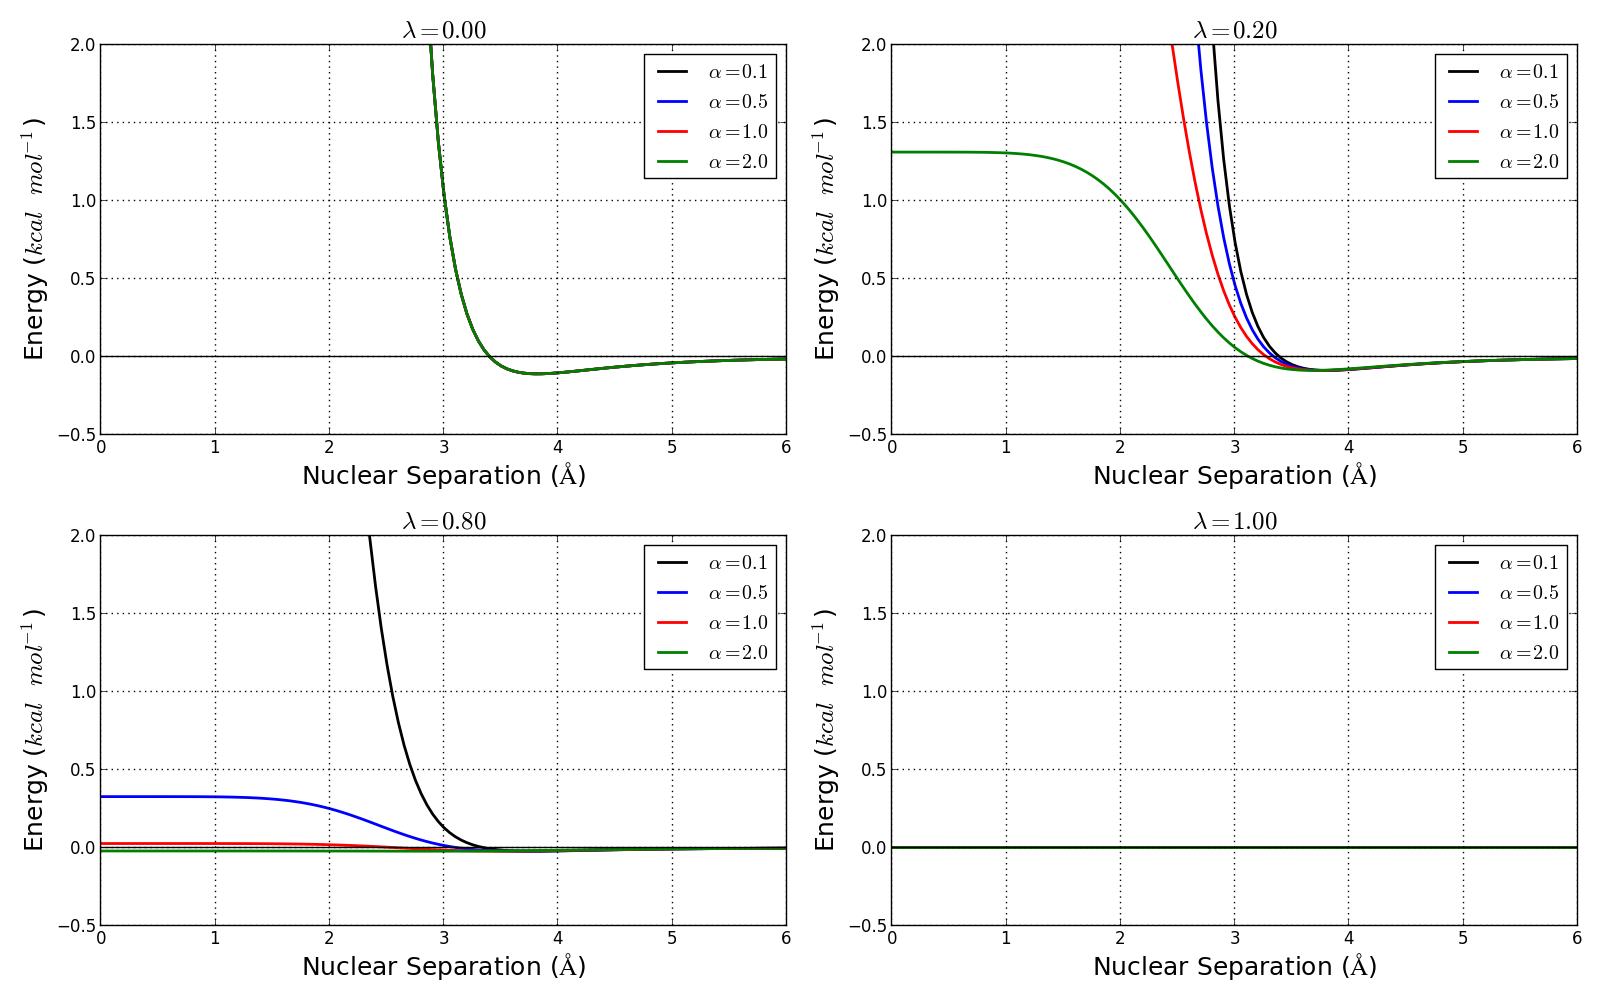
\includegraphics[width=6.5in, height=4.06in]{SoftCore.png}
   \caption[Functional form of soft-core Lennard Jones interactions with
            different values of $\alpha$ from Eq. \ref{eq2:SoftCore}.]
           {Functional form of soft-core Lennard Jones interactions with
            different values of $\alpha$ from Eq. \ref{eq2:SoftCore}. The
            $\lambda = 1$ state is the one in which an atom has vanished. See
            Fig. \ref{fig2:HardCore} to see how soft cores enable sampling close
            to the center of the vanishing atom when $\lambda \approx 1$.}
   \label{fig2:SoftCore}
\end{figure}

\subsection{Free Energy Perturbation}

An alternative approach to calculate the free energy difference between two
states is the free energy perturbation (FEP) method proposed by
\citeauthor{Zwanzig_JChemPhys_1954_v22_p1420}.
\cite{Zwanzig_JChemPhys_1954_v22_p1420} The free energy between two states A and
B can be calculated according to Eq. \ref{eq2:FEP}.

\begin{equation}
   \Delta G _ {A \rightarrow B} = -k_B T \ln \left \langle \exp \left( - \beta
         (E_B - E_A) \right) \right \rangle _ A
   \label{eq2:FEP}
\end{equation}
where the averages are taken over the ensemble generated in state $A$ and $E_B$
are the energies of the structures in ensemble $A$ evaluated with the
Hamiltonian governing the behavior of ensemble $B$. This is called
\emph{forward} sampling, since the ensemble we used to estimate the free energy
came from the original state. \cite{Leach_Book_MolModel_2001} The reverse, or
\emph{backward} sampling, represents the reverse process (\ie by swapping the
indices $A$ and $B$ in Eq. \ref{eq2:FEP}). Because free energy is a state
function, the forward and backward free energies should sum exactly to 0.

This balance between the forward and reverse sampling rarely balances completely
for complex transformations, however, indicating a shortcoming in the na\"ive
FEP approach. If the ensembles generated by the two states are significantly
different, the forward and reverse free energies will be systematically
different. For instance, if we are simulating the free energy change of
transforming benzene into phenol to calculate their difference in solvation free
energies, the solvent arrangement around the two systems will be significantly
different due to the added bulk of the hydroxyl group in phenol as well as the
difference in the dipole moment caused by that hydroxyl.

To address this shortcoming, two end-states are often interpolated using a
coupling parameter $\lambda$ similar in spirit to TI. By perturbing the system
slowly from state $A$ to $B$, the differences between adjacent states are
reduced, leading to similar ensembles that generate more consistent forward and
reverse free energies when used in Eq. \ref{eq2:FEP}.
\cite{Leach_Book_MolModel_2001}

\subsection{End-state Calculations}
\label{sec1:EndState}

The final family of free energy methods I will discuss here are so-called
\emph{end-state} calculations since they involve calculating the free energy
change $\Delta G_{A \rightarrow B}$ from simulations performed only on the two
physical end states $A$ and $B$. These methods are often used to estimate
binding free energies of a non-covalently bound protein-ligand or
protein-protein complex. \cite{Massova1999, Gohlke2003, Gohlke2004, Homeyer2012,
MMPBSApy}

I will discuss two methods within this family that are routinely used in binding
free energy calculations---the so-called Molecular Mechanics Poisson-Boltzmann
surface area (MM-PBSA) method \cite{Srinivasan_JAmChemSoc_1998_v120_p9401,
Massova2000} and the linear interaction energy (LIE) method.
\cite{Aqvist_ProteinEng_1994_v7_p385, Hansson1998}

\subsubsection{MM-PBSA}
\label{sec1:MMPBSA}

MM-PBSA, and its closely-related counterparts MM-GBSA (GB implicit solvent),
MM-3DRISM (3D-RISM implicit solvent), and QM/MM-GBSA, are commonly used to
calculate binding free energies of noncovalently bound complexes. These methods
compute binding free energies via the thermodynamic cycle shown in Fig.
\ref{fig2:MMPBSA}, where the solvation free energy terms are computed using an
implicit solvent model (\eg Poisson-Boltzmann, Generalized Born, or 3D-RISM).
The total free energy computed along the cycle, shown in Eq. \ref{eq2:MMPBSA},
is taken from ensemble averages over a simulated trajectory. The ensembles are
typically generated by running either a MD or MC simulation for each of the
three states---the bound complex, unbound receptor, and unbound ligand.
\cite{MMPBSApy}

\begin{equation}
   \Delta G_{binding} = \left \langle \Delta H_{solv,bound} \right \rangle +
      \left \langle \Delta H_{binding,gas} \right \rangle - \left \langle \Delta
      H_{solv, unbound} \right \rangle
   \label{eq2:MMPBSA}
\end{equation}
The averages in Eq. \ref{eq2:MMPBSA} are taken from the ensembles of each
system.

\begin{figure}
   \includegraphics[height=6.5in, angle=90]{MMPBSA.ps}
   \caption[Thermodynamic cycle for MM/PBSA calculations.]
           {Thermodynamic cycle for MM/PBSA calculations. Implicit solvent is
            represented with a blue background, while a white background
            represents systems in the gas phase.}
   \label{fig2:MMPBSA}
\end{figure}

The principle computational cost of an MM-PBSA calculation is due to the initial
simulations required to construct each ensemble. To reduce the cost of computing
binding free energies with MM-PBSA, all three ensembles mentioned above can be
extracted from a single simulation of the bound complex, a technique referred to
as the \emph{single trajectory protocol}. \cite{MMPBSApy} This approach will
always underestimate the binding free energy (predicting overly-stable binding),
since the bound states of the receptor and ligand will always be less stable in
the bound conformation than they are free in solution. However, when making the
same approximation for a family of related receptors and ligands, the systematic
errors in each end-state calculation will be similar. Therefore, MM-PBSA methods
can be useful for tasks like rank-ordering a handful of proposed inhibitors for
a specific enzyme by calculating accurate relative binding free energies.
\cite{Homeyer2012}

\subsubsection{LIE}

The linear interaction energy method (LIE) is another end-state method widely
used to calculate noncovalent binding free energies of small ligands to
proteins. LIE is based on assuming that the binding free energy is a result of
the energetic differences of the ligand in the two environments---bound in the
active site of the protein versus hydrated in solution---and obeys linear
response theory. \cite{Aqvist_ProteinEng_1994_v7_p385} The electrostatic
contribution to LIE can be simplified to the concept of charging the atoms of
the ligand inside a cavity that has the same shape as the ligand. Following the
ideas Marcus theory, \cite{Marcus1955} the reorganization energy of the
surrounding solvent $\lambda$ can be expressed as
\cite{Aqvist_ProteinEng_1994_v7_p385}
\begin{equation}
   \lambda = \left \langle V_B - V_A \right \rangle _ A - \Delta G _ {A
         \rightarrow B} = \left \langle V _ A - V _ B \right \rangle + \Delta G
         _ {A \rightarrow B}
   \label{eq2:Reorganization}
\end{equation}

Solving for $\Delta G _ {A \rightarrow B}$ in Eq. \ref{eq2:Reorganization}
yields the following expression for the free energy of the change from the
ligand bound in environment $A$ to the ligand bound in environment $B$:
\begin{equation}
   \Delta G _ {A \rightarrow B} = \frac 1 2 \left( \left \langle \Delta V
      \right \rangle _ A + \left \langle \Delta V \right \rangle _ B \right)
   \label{eq2:ReorganizationFE}
\end{equation}

Eq. \ref{eq2:ReorganizationFE} can be readily applied to the electrostatic
contribution of the binding free energy, but the non-polar non-bonded
interactions---namely the van der Waals interactions---are not known to obey
Marcus theory accurately. As a result, the non-polar interaction energy is
scaled in Eq. \ref{eq2:LIE} by a parameter that is adjusted to fit a database of
known binding affinities. \cite{Aqvist_ProteinEng_1994_v7_p385}

\begin{equation}
   \Delta G_{bind} = \frac 1 2 \left \langle \Delta V_{w \rightarrow p} ^{elec}
         \right \rangle + \alpha \left \langle \Delta V_{w \rightarrow p} ^{vdW}
         \right \rangle
   \label{eq2:LIE}
\end{equation}
where the `w' subscript indicates the ligand free in water and `p' indicates the
ligand bound in the protein. The van der Waals interactions are scaled by the
parameter $\alpha$, which was adjusted to give good agreement with experimental
binding affinities. LIE calculations require two ensembles to be generated---one
of the ligand free in explicit solvent and the other of the ligand bound in the
protein. A diagrammatic representation of the LIE calculation is shown in Fig.
\ref{fig2:LIE}.

\begin{figure}
   \includegraphics[height=6.5in, angle=90]{LIE.ps}
   \caption{Schematic showing interactions necessary to compute the LIE free
            energy of noncovalent binding for a ligand in a protein using white
            arrows.}
   \label{fig2:LIE}
\end{figure}
